\documentclass[beamer,dvipsnames]{standalone}

\usepackage{tikz}
\usetikzlibrary{positioning,decorations.pathreplacing,decorations.pathmorphing,arrows,fit}
\usetikzlibrary{calc}

\begin{document}

\begin{standaloneframe}[fragile]

\resizebox{\textwidth}{!}{

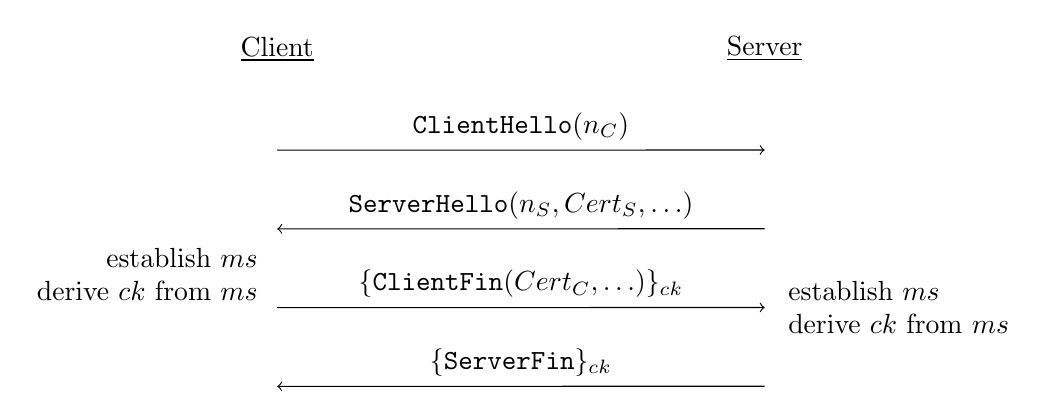
\begin{tikzpicture}
	\tikzset{
	    between/.style args={#1 and #2}{
	         at = ($(#1)!0.5!(#2)$)
	    }
	}
	

	\node (client) {\underline{Client}};
	\node[right=5cm of client] (server) {\underline{Server}};
	
	\coordinate[below = of client] (c1) {};
	\coordinate[below = 2 of client] (c2) {};
	\coordinate[below = 3 of client] (c3) {};
	\coordinate[below = 4 of client] (c4) {};
	\coordinate[below = of server] (s1) {};
	\coordinate[below = 2 of server] (s2) {};
	\coordinate[below = 3 of server] (s3) {};
	\coordinate[below = 4 of server] (s4) {};
	\coordinate[between = c4 and s4] (midpoint) {};
	
	\draw[->] (c1) -- node[above] {$\mathtt{ClientHello}(n_C)$} (s1);
	\draw[<-] (c2) -- node[above] {$\mathtt{ServerHello}(n_S, Cert_S, \dots)$} (s2);
	\draw[->] (c3) -- node[above] {$\lbrace \mathtt{ClientFin}(Cert_C, \dots) \rbrace_{ck}$} (s3);
	\draw[<-] (c4) -- node[above] {$\lbrace \mathtt{ServerFin} \rbrace_{ck}$} (s4);
	
	\node[below left = 5pt of c2,align=right] {establish $ms$\\derive $ck$ from $ms$};
	\node[right= 5pt of s3,align=left] {establish $ms$\\derive $ck$ from $ms$};
%	\node[left of= c4] {$\mathtt{accept}$};

%	\uncover<2-2>{
%		\node[draw, below=30pt of midpoint,inner sep = 5pt,align=center] {$ck \gets \mathsf{tls.PRF}(ms,``\mathtt{key\ expansion}", n_C \concat n_S)$};
%	}
%	
%	\uncover<3->{
%		\node[draw, below=30pt of midpoint,inner sep = 5pt,align=center] {$ck \gets \mathsf{tls.PRF}(ms,``\mathtt{key\ expansion}", n_C \concat n_S)$\\\textcolor{red}{$ek \gets \mathsf{tls.PRF}(ms,``\mathtt{some\ other\ label}", n_C \concat n_S)$}};
%	}
	
\end{tikzpicture}

}
\end{standaloneframe}

\end{document}